\clearpage
\subsection{Other Devices} % (fold)
\label{sub:other_devices}

The input/output operations are fairly standardised across different device types. Saving data to a file is very similar to writing it to the Terminal or to a network. The skills you learn with any one of these will be transferable to other devices.

\begin{figure}[h]
   \centering
   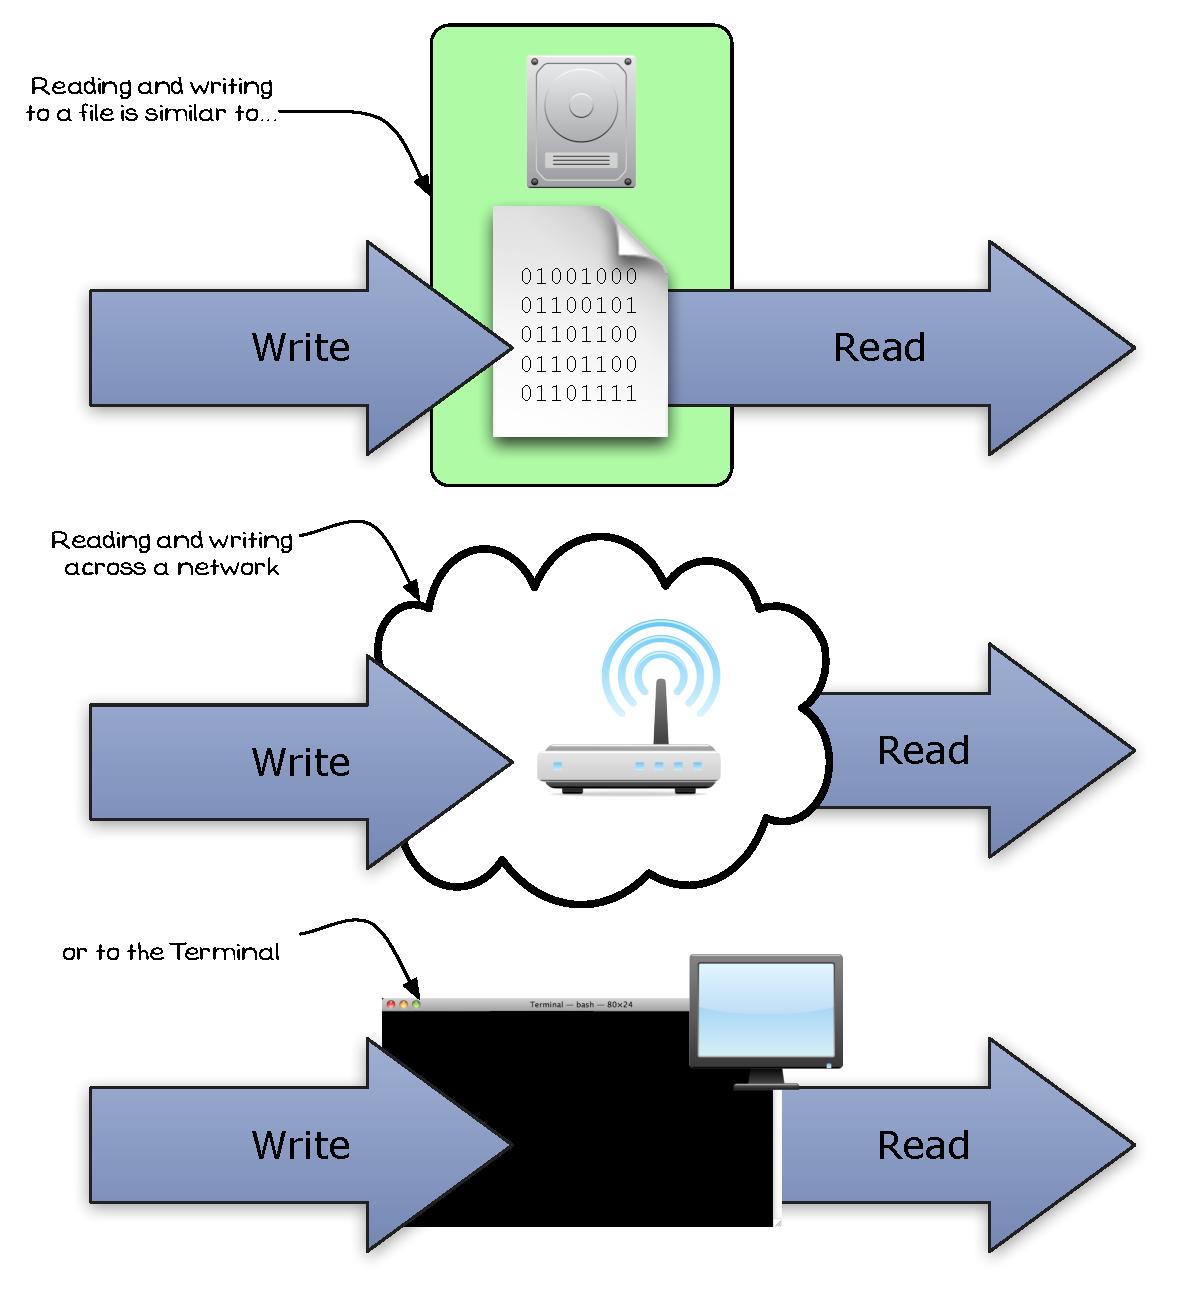
\includegraphics[width=0.9\textwidth]{./topics/file-io/diagrams/OtherDevices} 
   \caption{Writing to other devices also follows similar patterns}
   \label{fig:other-devices}
\end{figure}

\mynote{
\begin{itemize}
  \item The tasks you need to do to read and write data are similar, regardless of the destination device.
  \item Reading and writing to file is similar to reading and writing from the Terminal.
  \item You can open connections to other machines, and read and write data across these connections. Lookup details on sockets if you are interested in doing this.
\end{itemize}
}


% subsection other_devices (end)